\documentclass[11pt
  , a4paper
  , article
  , oneside
  %  , twoside
  , showtrims
 % , draft
]{memoir}

\usepackage{essdocs}
\usepackage[numbers]{natbib}
\usepackage[autostyle]{csquotes}

\setsecnumdepth{subsection}

\begin{document}
%\frontmatter
%% ESS Document Description
%%
\essdocdesc{Engineering Manual}

%% ESS Document Number
%%
\essdocnum{ESS-XXXXXXXX}

%% Date
%%
\date{\today}

%% ESS Document Revision Number
%%
\essdocrev{0.1}

%% ESS Document State
%%
\essdocstate{Early Draft}

%% ESS Document Classification
%%
\essdocclass{ESS Use Only}

%% Document Title
%%
\title{ICS Engineering Manual}
\subtitle{for MRF cPCI-EVG-230}
%% Document Author(s), if more than one author,
%% use \newline instead of \\ or \linebreak in order to seperate them
\author{Javier Cereijo Garcia \newline Jeong Han Lee }

%% Document Reviewer(s) if more than one reviewer,
%% use \newline instead of \\ or \linebreak in order to seperate them
%\reviewer{Timo Korhonen (Chief Engineer) \newline Timo Korhonen (Chief Engineer)}
\reviewer{TBD}
%% Document Owner(s) if more than one owner,
%% use \newline instead of \\ or \linebreak in order to seperate them
\owner{ICS}

%% Document Approver(s) if more than one approver,
%% use \newline instead of \\ or \linebreak in order to seperate them
\approver{ICS}

\showtrimson

\esstitle
\newpage
\tableofcontents
\newpage

%\mainmatter


%%% Actual Document Start at below
\chapter{Overview}
At European Spallation Source (ESS), Integrated Control System (ICS) does use the Micro Research Finland (MRF) Timing System{\footnote{\url{http://www.mrf.fi/}}} as its timing system of the ESS site. The consistent and up-to-date engineering manual is essential for the ESS Timing system.

\section{Scope}
\begin{itemize}
\item This document identifies one of the MRF Timing Event Receivers (EVR) that needs to be configured for an ESS subsystem that needs synchronous frequencies, trigger signals and sequences of events \cite{MRFEVENTSYSTEMDC}.
\item This document provides the generic description of the MRF PCIe-EVR-300 and its interface board (IFB-300). In addition, it affords the minimal, essential, and generic information for the system configuration.  
\item The purpose of this document is to describe the engineering procedure and troubleshooting about how the MRF PCIe-EVR-300 board will be integrated in cooperation with the ESS EPICS Environment (EEE).
\item This document attempts to maintain consistency with existing ESS Timing system hardware as far as possible. 
\end{itemize}
\textbf{Note that this is a very early draft document and should be updated as development progresses.}

\section{Target Audience}
This document is targeted to ICS engineers and technical stakeholders of the ESS timing system. It is assumed that the target audience has a technical background in the MRF Timing System, the EPICS development, and a Linux environment.

\chapter{System Description}
MRF Technical Reference \citep[see][p45]{MRFEVENTSYSTEMDC} explained Event Receivers and wrote :
\blockquote{\textit{Event Receivers decode timing events and signals from an optical event stream transmitted by an Event Generator. Events and signals are received at predefined rate the event clock that is usually divided down from an accelerators main RF reference. The event receivers lock to the phase event clock of the Event Generator and are thus phase locked to the RF reference. Event Receivers convert event codes transmitted by an Event Generator to hardware outputs. They can also generate software interrupts and store the event codes with globally distributed timestamps into FIFO memory to be read by a CPU.}}

ICS uses and will use the following different types of EVR :
\begin{itemize}
\item VME-EVR-230 / 230RF
\item PMC-EVR-230
\item mTCA-EVR-300 / 300DC
\item PCIe-EVR-300 / 300DC
\item VME-EVR-300 / 300DC
\end{itemize}

And the scope of this document is to cover PCIe-EVR-300 board, PCIe-EVR-300DC\footnote{Delay Compensation (DC) Unit. Currently we only use the EVR-300 board in this document.} board, or both boards.


\section{PCIe-EVR-300DC}
Figure~\ref{fig:pcie-evr300dc} shows the rough physical dimensions $104\times 79~\mathrm{mm}{}^2$ of the PCIe-EVR-300DC card, which  will replace the former PCIe-EVR-300. And its power dissipation is almost 10W, so one should check the maximum power of each PCIe slot where the card will be. And it is advisable to have some forced cooling method to keep the temperature of the card reasonable \citetext{priv. comm.}.

\begin{figure}[!htb]
  \centering
  \includegraphics[width=0.99\textwidth]{./pictures/pcie_evr_300dc.eps}
  \caption{
    MRF PCIe-EVR-300 with Delay Compensation Unit.
  }
  \label{fig:pcie-evr300dc}   
\end{figure}


The PCIe-EVR-300  has a SFP transceiver as an input from EVG and a micro-SCSI type connector as an output to subsystem, because of its small form factor \cite{MRFEVENTSYSTEMDC}. Thus, in order to send supported type of signals to a subsystem, the interface board IFB-300 is needed. The IFB-300 has eight Universal I/O slots, shown in Figure~\ref{fig:ifb-300}. With different type of MRF Universal I/O modules, each slot can be used as an unique trigger or event signal source.

\begin{figure}[!htb]
  \centering
  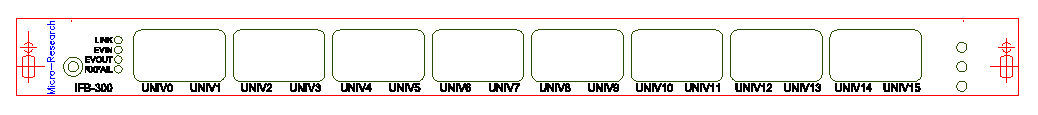
\includegraphics{./pictures/ifb-300.eps}
  \caption{
    MRF Interface Board IFB 300 Front Panel \cite{MRFEVENTSYSTEMDC}.
  }
  \label{fig:ifb-300}   
\end{figure}


\clearpage

\chapter{System Environment}
Before describing the engineering procedure for an EEE integration of the MRF PCIe-EVR-300 board, it is mandatory to have proper system environment that consists of specific hardware and software lists. Here we will show the hardware and software lists, their block diagrams, and their setup in the ICS lab at ESS. The information shown in this chapter is used in the ICS Lab at ESS.


\section{Hardware}
Table~\ref{table:hwlist} shows the hardware list and its environment. The form factor and version of EVG can be changeable. It is assumed that the proper working EVG system is ready. Here, \texttt{TAG} is used as the prefix of the ICS internal inventory system in order to track it down. One can use only EVG without FOUT. Kontron Industrial PC can be able to replace with PC, workstation, or server with a compatible PCIe slot. Note that this PCIe slot for the MRF PCIe-EVR-300 should support more than 10W.
\begin{table}[!hb]
  \centering
  \begin{tabular}{l|l|l}
    \toprule
    Hardware                  & Info                   & Serial Number \\\midrule
    MRF PCIe-EVR-300          & \texttt{ICS TAG-146}   & K114029       \\\midrule
    Kontron Industrial PC     & Hostname : ics-essiip-01&              \\\midrule
    MRF IFB-300               & \texttt{ICS TAG-336}   & K472056       \\\midrule
    Universal I/O             &                        &               \\\midrule
    MRF cPCI-EVG-230          & \texttt{ICS TAG-26}    & E283016       \\\midrule
    MRF cPCI-FOUT-12          & \texttt{ICS TAG-27}    & H385013       \\\midrule
    Optical cables            & LC, Optical 850 nm     &               \\\midrule
    LEMO cables               &                        &               \\\midrule
    LEMO to BNC Adapters      &                        &               \\\midrule
    Oscilloscope              &                        &               \\\bottomrule
  \end{tabular}
  \caption[]{Hardware List and Its Environment.}
  \label{table:hwlist}
\end{table}


Figure~\ref{fig:diagram} shows the physical hardware setup and Figure~\ref{fig:hw-setup} shows the PCIe-MRF-300 and the IFB-300 setup in the lab. 
\begin{figure}[!t]
  \centering
    \includegraphics[width=0.7\textwidth]{./pictures/pcie_network.eps}
  \caption{Hardware setup diagram}
  \label{fig:diagram}
\end{figure}
\begin{figure}[!b]
  \centering
  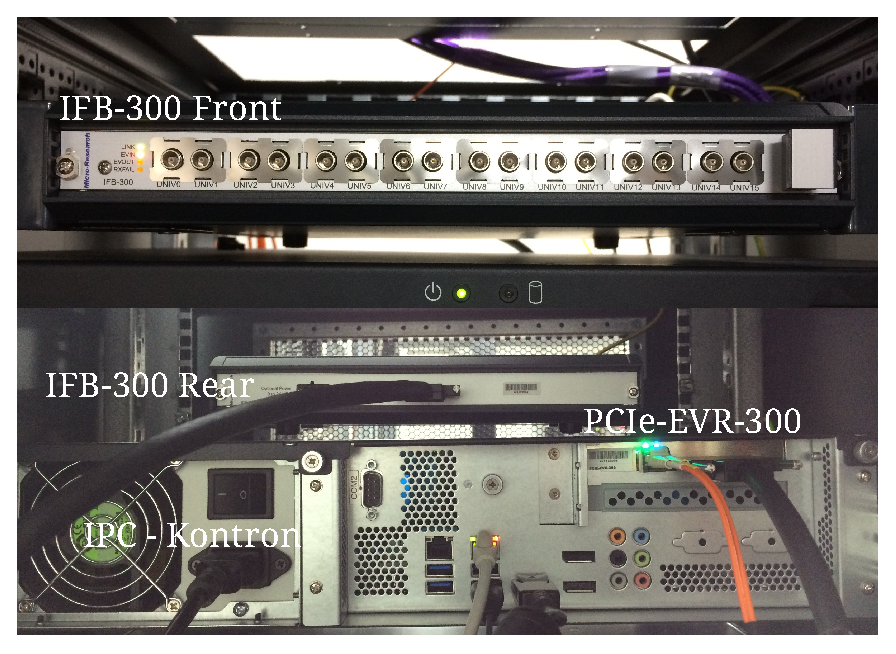
\includegraphics[width=0.8\textwidth]{./pictures/hw-setup.eps}
  \caption{Hardware Setup in the ICS lab.}
  \label{fig:hw-setup}   
\end{figure}


\clearpage
\section{Software}
Table~\ref{table:swlist} shows the Software list and its environment. It is mandatory to check the kernel version, and the mrf kernel module version. Since the mrfioc2 is dependent upon devLibs2 EEE internally, an end-user is unnecessary to check its version explicitly. 
\begin{table}[!htb]
  \centering
  \begin{tabular}{l|l}
    \toprule
    Item               & Version Info.                                            \\\midrule
    CentOS Linux       & \texttt{7.1.1503}                                        \\\midrule
    Kernel             & \texttt{3.10.0-229.7.2.rt56.141.6.el7.centos.x86\_64}    \\\midrule
    mrf kernel module  & version : \texttt{1} / srcversion \texttt{124F2C1F3D5E2080AE1B755}     \\\midrule
    EEE                & \texttt{1.8.0}                                  \\\midrule
    EPICS Base         & \texttt{3.14.12.5}                              \\\midrule
    mrfioc2            & EEE module ver. \texttt{3.0.0}                  \\\midrule
    devLib2            & EEE module ver. \texttt{2.6+}                   \\\bottomrule
  \end{tabular}
  \caption[]{Software and its version information.}
  \label{table:swlist}
\end{table}

\section{EVR Firmware}
Table~\ref{table:fwinfo} shows EVR FPGA Firmware Version Register.
%Note that the EVR Revision ID of the MRF PCIe-EVR-300 in the ICS Lab is not in Reference \cite{MRFEVENTSYSTEMDC}.

\begin{table}[!htb]
  \centering
  \begin{tabular}{p{0.3\linewidth}|c|l}
    \toprule
    EVR FPGA Firmware Version Register            & \multicolumn{2}{c}{\texttt{0x17000008}}             \\\midrule
    Board Type      & EVR                         &  \texttt{0x}\underline{\textbf{1}}\texttt{7000008}  \\\midrule
    Form Factor     & PCIe                        &  \texttt{0x1}\underline{\textbf{7}}\texttt{000008}  \\\midrule
    EVR Firmware ID & Modular Register Map (MRM)  &  \texttt{0x1700}\underline{\textbf{00}}\texttt{08}  \\\midrule
    EVR Revision ID & 8                           &  \texttt{0x170000}\underline{\textbf{08}}           \\\bottomrule
  \end{tabular}
  \caption[]{EVR FPGA Firmware Version Register in Reference \citep[see][p66]{MRFEVENTSYSTEMDC}. The EVR in the ICS Lab does not have the Delay Compensation firmware, but the Modular Register Map firmware.}
  \label{table:fwinfo}
\end{table}


\clearpage
\chapter{Engineering Procedure}
This chapter provides the minimal information to configure the EVR board properly. 

\section{System Installation}
Figure~\ref{fig:diagram} and Figure~\ref{fig:hw-setup} shows the glimpse of what system might be like in a Lab. \textbf{Note that the cable between the PCIe-EVR-300DC and IFB-300 should be connected, disconnected, or both only when powered down}. Please see the detail information in Reference \citep[][p54]{MRFEVENTSYSTEMDC}.
  
\section{PCIe EVR-300 Board Identification}
         
\subsection{Kernel Module}
It is essential to load the mrf kernel module and to check its information as follows:
\begin{lstlisting}[style=termstyle]
root@ics-essiip-01:~# modprobe mrf
  
root@ics-essiip-01:~# modinfo mrf
filename:       /lib/modules/3.10.0-229.7.2.rt56.141.6.el7.centos.x86_64/extra/mrf.ko
author:         Michael Davidsaver <mdavidsaver@bnl.gov>
version:        1
license:        GPL v2
rhelversion:    7.1
srcversion:     124F2C1F3D5E2080AE1B755
depends:        parport,uio
vermagic:       3.10.0-229.7.2.rt56.141.6.el7.centos.x86_64 SMP preempt mod_unload modversions 
parm:           cable:Name of JTAG parallel port cable to emulate (charp)
parm:           interfaceversion:User space interface version (int)
\end{lstlisting}

It is mandatory to check the access permission of an IOC user for the device file, e.g., \path{/dev/uio0} to allow the IOC process to open it. In case ones target system is NOT running \texttt{UDEV}, please consult the EVG user guide~\cite{EVR-USER-GUIDE}. And for building and loading the EVR kernel module and for changing the device file permission, please see Reference~\citep[see][p12,13]{EVR-USER-GUIDE}. It is inadvisable to change the file permission by using \texttt{chmod}. 

\subsection{PCI Addressing}
Each PCI device is identified by a domain, a bus, a device, and a function number in Linux. Therefore, in order to initialize the MRF PCIe-EVR-300 board in EEE, one needs the following information: a domain number, a bus number, a device number, and a function number. These numbers are the parameters of a \texttt{mrmEvrSetupPCI} function.

One can use \texttt{lspci} to find them as follows:
\begin{lstlisting}[style=termstyle]
  root@ics-essiip-01:~# lspci
  05:00.0 Signal processing controller: Lattice Semiconductor Corporation Device ec30 (rev 01)

  root@ics-essiip-01:~# lspci -s 05:00 -vv
  05:00.0 Signal processing controller: Lattice Semiconductor Corporation Device ec30 (rev 01)
	Subsystem: Device 1a3e:172c
	Control: I/O+ Mem+ BusMaster+ SpecCycle- MemWINV- VGASnoop- ParErr- Stepping- SERR- FastB2B- DisINTx-
	Status: Cap+ 66MHz- UDF- FastB2B- ParErr- DEVSEL=fast >TAbort- <TAbort- <MAbort- >SERR- <PERR- INTx-
	Latency: 0, Cache Line Size: 64 bytes
	Interrupt: pin A routed to IRQ 16
	Region 0: Memory at c0400000 (32-bit, non-prefetchable) [size=1M]
	Capabilities: [50] Power Management version 3
		Flags: PMEClk- DSI- D1- D2- AuxCurrent=0mA PME(D0-,D1-,D2-,D3hot-,D3cold-)
		Status: D0 NoSoftRst- PME-Enable- DSel=0 DScale=0 PME-
	Capabilities: [70] MSI: Enable- Count=1/1 Maskable- 64bit+
		Address: 0000000000000000  Data: 0000
	Capabilities: [90] Express (v1) Endpoint, MSI 00
		DevCap:	MaxPayload 128 bytes, PhantFunc 0, Latency L0s <64ns, L1 <1us
			ExtTag- AttnBtn- AttnInd- PwrInd- RBE+ FLReset-
		DevCtl:	Report errors: Correctable- Non-Fatal- Fatal- Unsupported-
			RlxdOrd+ ExtTag- PhantFunc- AuxPwr- NoSnoop-
			MaxPayload 128 bytes, MaxReadReq 512 bytes
		DevSta:	CorrErr- UncorrErr- FatalErr- UnsuppReq- AuxPwr- TransPend-
		LnkCap:	Port #0, Speed 2.5GT/s, Width x1, ASPM L0s, Exit Latency L0s unlimited, L1 <1us
			ClockPM- Surprise- LLActRep- BwNot-
		LnkCtl:	ASPM Disabled; RCB 64 bytes Disabled- CommClk+
			ExtSynch- ClockPM- AutWidDis- BWInt- AutBWInt-
		LnkSta:	Speed 2.5GT/s, Width x1, TrErr- Train- SlotClk+ DLActive- BWMgmt- ABWMgmt-
	Capabilities: [100 v1] Vendor Specific Information: ID=0000 Rev=0 Len=00c <?>
	Kernel driver in use: mrf-pci
\end{lstlisting}

And one should identify four number as follows:
\begin{lstlisting}[style=termstyle]
  root@ics-essiip-01:~# lspci -s 05:00 -t
  -+-[0000:05]---00.0
  \-[0000:00]-
\end{lstlisting}
, where \texttt{-+-[0000:05]---00.0} can be translated to \texttt{-+-}[domain:bus]\texttt{---}device.function. Thus in the above case, four numbers are shown in Table~\ref{table:pciidnumber}.\begin{table}[!htb]
  \centering
  \begin{tabular}{l|l}
    \toprule
    domain   & 0x0 \\\midrule
    bus      & 0x5 \\\midrule
    device   & 0x0 \\\midrule
    function & 0x0 \\\bottomrule
  \end{tabular}
  \caption[]{MRF PCIe-EVR-300 Identification Numbers}
  \label{table:pciidnumber}
\end{table}


\clearpage
\section{EPICS IOC Setup under EEE}
In this section, in order to start the EPICS IOC for the MRF PCIe-EVR-300 under EEE, one should consider the following things: 1) the EPICS database file, and 2) the EPICS start-up script. All files are located in a directory, where an user can create, e.g., in the ICS Lab, 
\begin{lstlisting}[style=termstyle, label={list:pwd}, caption={Working Directory in the ICS lab.} ]
  /home/javiercereijogarcia/PCIe-EVR-300_tests
\end{lstlisting}

\subsection{EPICS Database File}
One could use the existent database file in the EEE as a template for the EPICS IOC, the file is located in the following location : 
\begin{lstlisting}[style=termstyle]
  /opt/epics/modules/mrfioc2/3.0.0/db/evr-pcie-300.db
\end{lstlisting}

In the ICS Lab, the event clock frequency of the event generator (EVG) is set to 88.0525 MHz and the EVG sends the event number 14, at 14 Hz to the EVR. The link clock frequency in the database file of the EVR should be matched to the EVG event clock frequency. Thus, one should change the hardcode of \texttt{Link-Clk-SP} from the existent line \ref{oldlinkclockfreq} to  the modified line \ref{newlinkclockfreq} in Listing~\ref{list:record}. 
\begin{lstlisting}[style=termstylenumber, label={list:record}, caption={The record has the link clock frequency.}] 
  record(ao, "$(SYS,recursive)-$(EVR,recursive):Link-Clk-SP")
  {
    field(DTYP, "Obj Prop double")
    field( OUT, "@OBJ=$(EVR,recursive), PROP=Clock")
    field(PINI, "YES")
    field(DESC, "Event Link speed")
-   field( VAL, "$(Link-Clk-SP=124.916(*@\label{oldlinkclockfreq}@*), undefined)")}
+   field( VAL, "$(Link-Clk-SP=88.0525(*@\label{newlinkclockfreq}@*), undefined)")}
    field(EGU , "MHz")
    field(LINR, "LINEAR")
    field(ESLO, "1e-6")
    field(HOPR, "150")
    field(LOPR, "50")
    field(DRVH, "150")
    field(DRVL, "50")
    field(PREC, "3")
    field(FLNK, "$(SYS,recursive)-$(EVR,recursive):Link-Clk-I")
    info(autosaveFields_pass0, "VAL EGU ESLO HOPR LOPR DRVH DRVL PREC")
  }
\end{lstlisting}
Note that one can also change this Process Variable \texttt{Link-Clk-SP} when the IOC is started. 


\subsection{Start-Up Script}
Listing~\ref{list:st.cmd} shows the IOC start-up script which has the MRF PCIe-EVR-300 Identification Numbers, shown in Table~\ref{table:pciidnumber}. Note that the start-up script is located in the directory in Listing~\ref{list:pwd}. Moreover, the database file, \texttt{evr-pcie-300.db}, path must be in the current directory (\path{./}) in Line \ref{dbpwd}.


\begin{lstlisting}[
    style=termstylenumber,
    label={list:st.cmd},
    caption={Start-up script \texttt{evr300\_0.cmd}. Line \ref{pciid0}-\ref{pciid3} should be matched to Table~\ref{table:pciidnumber}. }
  ]
  epicsEnvSet("SYS"             "SYS0")
  epicsEnvSet("EVR"             "EVR0")
  epicsEnvSet("EVR_PCIDOMAIN"   "0x0") (*@\label{pciid0}@*)
  epicsEnvSet("EVR_PCIBUS"      "0x5") (*@\label{pciid1}@*)
  epicsEnvSet("EVR_PCIDEVICE"   "0x0") (*@\label{pciid2}@*)
  epicsEnvSet("EVR_PCIFUNCTION" "0x0") (*@\label{pciid3}@*)
  
  require mrfioc2
  
  mrmEvrSetupPCI($(EVR), $(EVR_PCIDOMAIN), $(EVR_PCIBUS), $(EVR_PCIDEVICE), $(EVR_PCIFUNCTION))
  
  dbLoadRecords("./evr-pcie-300.db", "EVR=$(EVR), SYS=$(SYS)") (*@\label{dbpwd}@*)
  
\end{lstlisting}

\subsection{EPICS IOC}
Under EEE, the EPICS IOC can be started via the command \texttt{iocsh evr300\_0.cmd}. The output should look like as follows:

\begin{lstlisting}[style=termstyle]
  [javiercereijogarcia@ics-essiip-01 PCIe-EVR-300_tests]$ iocsh evr300_0.cmd 
  /opt/epics/bases/base-3.14.12.5/bin/centos7-x86_64/softIoc -D /opt/epics/bases/base-3.14.12.5/dbd/softIoc.dbd /tmp/iocsh.startup.20268
  #date="Fri 15 Jul 15:55:53 UTC 2016"
  #user="javiercereijogarcia"
  #PWD="/home/javiercereijogarcia/PCIe-EVR-300_tests"
  #EPICSVERSION="3.14.12.5"
  #EPICS_HOST_ARCH="centos7-x86_64"
  #SHELLBOX=""
  #EPICS_CA_ADDR_LIST=""
  #EPICS_MODULE_INCLUDE_PATH=".:/usr/lib64:/usr/lib:/lib64:/lib"
  dlload         /opt/epics/modules/environment/1.8.0/3.14.12.5/lib/centos7-x86_64/libenvironment.so
  dbLoadDatabase /opt/epics/modules/environment/1.8.0/3.14.12.5/dbd/environment.dbd
  environment_registerRecordDeviceDriver
  < "evr300_0.cmd"
  epicsEnvSet("SYS"             "SYS0")
  epicsEnvSet("EVR"             "EVR0")
  epicsEnvSet("EVR_PCIDOMAIN"   "0x0")
  epicsEnvSet("EVR_PCIBUS"      "0x5")
  epicsEnvSet("EVR_PCIDEVICE"   "0x0")
  epicsEnvSet("EVR_PCIFUNCTION" "0x0")
  require mrfioc2
  require: mrfioc2 depends on devlib2 (2.6+).
  require: Loading library /opt/epics/modules/devlib2/2.6.0/3.14.12.5/lib/centos7-x86_64/libdevlib2.so.
  require: Loading /opt/epics/modules/devlib2/2.6.0/3.14.12.5/dbd/devlib2.dbd.
  require: Calling devlib2_registerRecordDeviceDriver function.
  require: Loading library /opt/epics/modules/mrfioc2/3.0.0/3.14.12.5/lib/centos7-x86_64/libmrfioc2.so.
  require: Adding /opt/epics/modules/mrfioc2/3.0.0/db.
  require: Adding /opt/epics/modules/mrfioc2/3.0.0/startup.
  require: Loading /opt/epics/modules/mrfioc2/3.0.0/3.14.12.5/dbd/mrfioc2.dbd.
  require: Calling mrfioc2_registerRecordDeviceDriver function.
  
  mrmEvrSetupPCI(EVR0, 0x0, 0x5, 0x0, 0x0)
  Device EVR0  5:0.0
  Using IRQ 16
  Setting magic LE number!
  EC 30: Enabling interrupts
  FWVersion 0x17000008
  Found version 8
  Found EVR0:SFP0 EEPROM
  PCIe: Out FP:0 FPUNIV:16 RB:0 IFP:0 GPIO:0
  EVR FIFO task start
  dbLoadRecords("./evr-pcie-300.db", "EVR=EVR0, SYS=SYS0")
  iocInit
  Starting iocInit
  ############################################################################
  ## EPICS R3.14.12.5-2015-08 $Date: Tue 2015-03-24 09:57:35 -0500$
  ## EPICS Base built Oct  9 2015
  ############################################################################
  Set EVR clock 88052500.000000
  cas warning: Configured TCP port was unavailable.
  cas warning: Using dynamically assigned TCP port 48729,
  cas warning: but now two or more servers share the same UDP port.
  cas warning: Depending on your IP kernel this server may not be
  cas warning: reachable with UDP unicast (a host's IP in EPICS_CA_ADDR_LIST)
  iocRun: All initialization complete
  epicsEnvSet IOCSH_PS1,"ics-essiip-01> "
  ics-essiip-01>
\end{lstlisting}

In addition, the PCI information is available within the running IOC via \texttt{devPCIShow} as follows:
\begin{lstlisting}
  ics-essiip-01> devPCIShow
  Look for the line with your configuration information, in our case is:
  PCI 0000:05:00.0 IRQ 16
    vendor:device 1204:ec30 rev 00
  Where the vendor id 1204 is Lattice.
  And show the PCI information with (the second parameter is the verbosity level):

  ics-essiip-01> devPCIShow 9 0x1204
  PCI 0000:05:00.0 IRQ 16
    vendor:device 1204:ec30 rev 00
    subved:subdev 1a3e:172c
    class 118000 generic signal processing controller
    driver mrf-pci
    BAR 0 32-bit MMIO      1 MB
    Matched 1 devices

  ics-essiip-01>
\end{lstlisting}

\newpage
\chapter{System In-Situ Verification Procedure}
This chapter provides the minimal system verification procedure. If one wants to do more step-by-step procedure which may be useful when testing the function of hardware and software, please see Reference~~\citep[see][p14]{EVR-USER-GUIDE}.

\begin{table}[!htb]
  \centering
  \begin{tabular}{c|p{0.4\linewidth}|p{0.42\linewidth}}
    \toprule
    Step & Goal                                       & Info.                                                  \\\midrule
    0    & Check the EVR \& EVR connection            & Link status, link clock, and heartbeat timeout counter \\\midrule
    1    & Monitor Receiving and acknowledging Events & Event counter and receiving event frequency            \\\midrule
    2    & Generate Trigger Signals from EVR          & Various trigger signals with an oscilloscope           \\\bottomrule
  \end{tabular}
  \caption[]{System In-Situ Verification Procedure}
  \label{table:checklist}
\end{table}


\section{Step 1 : Check the EVR and EVR connection}
Short comments on each command or a series of commands are shown before the corresponding command.
\begin{lstlisting}[style=termstyle]
  #
  # We can check the EVG and EVR link status and the link clock setting,
  # and can also see the link down counter as well.
  #
  user@host:~$ caget SYS0-EVR0:Link-Sts
  SYS0-EVR0:Link-Sts             OK
  user@host:~$ caget SYS0-EVR0:Link-Clk-I
  SYS0-EVR0:Link-Clk-I           88.0519
  #
  # change the wrong clock setting on EVR, then we expect that the link status will be Fail.  
  #
  user@host:~$ caput SYS0-EVR0:Link-Clk-SP 100
  Old : SYS0-EVR0:Link-Clk-SP          88.0525
  New : SYS0-EVR0:Link-Clk-SP          100
  user@host:~$ caget SYS0-EVR0:Link-Sts
  SYS0-EVR0:Link-Sts             Fail
  user@host:~$ caget SYS0-EVR0:Link-Clk-I
  SYS0-EVR0:Link-Clk-I           100
  #
  # revert it back to the proper clock setting, and the link status will be OK.
  #
  user@host:~$ caput SYS0-EVR0:Link-Clk-SP 88.0525
  Old : SYS0-EVR0:Link-Clk-SP          100
  New : SYS0-EVR0:Link-Clk-SP          88.0525
  user@host:~$ caget SYS0-EVR0:Link-Sts
  SYS0-EVR0:Link-Sts             OK
  user@host:~$ caget SYS0-EVR0:Link-Clk-I
  SYS0-EVR0:Link-Clk-I           88.0519

  #
  # The link heartbeat counter is 18
  #
  user@host:~$ camonitor SYS0-EVR0:Cnt-LinkTimo-I
  SYS0-EVR0:Cnt-LinkTimo-I       2016-06-30 10:23:23.949149 18

  #
  # open another terminal, to change the wrong link clock. 
  #
  # In another terminal:
  user@host:~$ caput SYS0-EVR0:Link-Clk-SP 100
  Old : SYS0-EVR0:Link-Clk-SP          88.0525
  New : SYS0-EVR0:Link-Clk-SP          100

  #
  # so, the heartbeat counter should be increasing as follows: 
  #
  SYS0-EVR0:Cnt-LinkTimo-I       2016-06-30 10:24:12.037271 19
  SYS0-EVR0:Cnt-LinkTimo-I       2016-06-30 10:24:13.735983 20
  SYS0-EVR0:Cnt-LinkTimo-I       2016-06-30 10:24:15.438585 21
  SYS0-EVR0:Cnt-LinkTimo-I       2016-06-30 10:24:17.137761 22
  SYS0-EVR0:Cnt-LinkTimo-I       2016-06-30 10:24:18.836612 23

  # the counter will be stopped after the proper value is given.
  # In another terminal:
  user@host:~$ caput SYS0-EVR0:Link-Clk-SP 88.0525
  Old : SYS0-EVR0:Link-Clk-SP          100
  New : SYS0-EVR0:Link-Clk-SP          88.0525
\end{lstlisting}

\section{Step 2 : Monitor Receiving and acknowledging Events}
For this step, an additional EVR database file is needed to add to the end line of the \path{evr300_0.cmd} file. This additional database file is located in \path{/opt/epics/modules/mrfioc2/3.0.0/db} and no modification is needed. The new start-up script file, \path{evr300_1.cmd} is shown in Listing~\ref{list:evr300-1.cmd}. Note that Line \ref{dbpwd2} show the current directory \path{./}. And Line \ref{dbsoftevtpwd} shows no path of the database file, because it can be detected automatically. 
\begin{lstlisting}[
    style=termstylenumber,
    label={list:evr300-1.cmd},
    caption={Start-up script \texttt{evr300\_1.cmd}. }
  ]
  epicsEnvSet("SYS"             "SYS0")
  epicsEnvSet("EVR"             "EVR0")
  epicsEnvSet("EVR_PCIDOMAIN"   "0x0") 
  epicsEnvSet("EVR_PCIBUS"      "0x5") 
  epicsEnvSet("EVR_PCIDEVICE"   "0x0") 
  epicsEnvSet("EVR_PCIFUNCTION" "0x0") 
  
  require mrfioc2
  
  mrmEvrSetupPCI($(EVR), $(EVR_PCIDOMAIN), $(EVR_PCIBUS), $(EVR_PCIDEVICE), $(EVR_PCIFUNCTION))
    
  dbLoadRecords("./evr-pcie-300.db",      "EVR=$(EVR), SYS=$(SYS)") (*@\label{dbpwd2}@*)
  dbLoadRecords("evr-softEvent.template", "EVR=$(EVR), SYS=$(SYS), EVT=14, CODE=14") (*@\label{dbsoftevtpwd}@*)
\end{lstlisting}

Short comments on each command or a series of commands are shown before the corresponding command.

\begin{lstlisting}[style=termstylenumber]
  #
  # start the IOC
  #
  user@host:~$ iocsh evr300_1.cmd

  #
  # monitor the Event counter with 14. and check the time difference between counters, e.g., 132 and 133, is 0.071429s, i.e., 14 Hz.
  # In another terminal:
  user@host:~$ camonitor SYS0-EVR0:Event-14-Cnt-I
  SYS0-EVR0:Event-14-Cnt-I       2016-06-30 13:55:36.008609 132
  SYS0-EVR0:Event-14-Cnt-I       2016-06-30 13:55:36.080038 133
  SYS0-EVR0:Event-14-Cnt-I       2016-06-30 13:55:36.151467 134
  SYS0-EVR0:Event-14-Cnt-I       2016-06-30 13:55:36.222895 135
  SYS0-EVR0:Event-14-Cnt-I       2016-06-30 13:55:36.294324 136
\end{lstlisting}


\section{Step 3 : Generate Trigger Signals from EVR}
For this step, an additional EVR database file with two configrations is also needed to add to the end line of the \path{evr300_1.cmd} file. This additional database file is located in \path{/opt/epics/modules/mrfioc2/3.0.0/db}, and no modification is needed. Thus, the new start-up script file, \path{evr300_2.cmd} is shown in Listing~\ref{list:evr300-2.cmd}. Note that each path of database files should be checked correctly. 
\begin{lstlisting}[ 
    style=termstylenumber,
    label={list:evr300-2.cmd},
    caption={Start-up script \texttt{evr300\_2.cmd}.}
  ]
  epicsEnvSet("SYS"             "SYS0")
  epicsEnvSet("EVR"             "EVR0")
  epicsEnvSet("EVR_PCIDOMAIN"   "0x0")
  epicsEnvSet("EVR_PCIBUS"      "0x5")
  epicsEnvSet("EVR_PCIDEVICE"   "0x0")
  epicsEnvSet("EVR_PCIFUNCTION" "0x0")
  
  require mrfioc2
  
  mrmEvrSetupPCI($(EVR), $(EVR_PCIDOMAIN), $(EVR_PCIBUS), $(EVR_PCIDEVICE), $(EVR_PCIFUNCTION))
  
  dbLoadRecords("./evr-pcie-300.db",      "EVR=$(EVR), SYS=$(SYS)")
  dbLoadRecords("evr-softEvent.template", "EVR=$(EVR), SYS=$(SYS), EVT=14, CODE=14") 
  dbLoadRecords("evr-pulserMap.template", "EVR=$(EVR), SYS=$(SYS), PID=0, F=Trig, ID=0, EVT=14")
  dbLoadRecords("evr-pulserMap.template", "EVR=$(EVR), SYS=$(SYS), PID=1, F=Trig, ID=0, EVT=14")
\end{lstlisting}

An EVR is composed of several logical sub-units, and one of the logical sub-units is the pulse generator. And each pulse generator has an associated Delay and Width \cite{EVR-USER-GUIDE}. In the following procedure, two pulse generators are mapped to the \path{UNIV0} and \path{UNIV1} of IFB-300, which are connected to the channel 1 and 2 of the oscilloscope respectively in order to see whether output signals are generated according to Delay's and Width's changes. Short comments on each command or a series of commands are shown before the corresponding command.

\subsection{\texttt{UNIV0} output}
\begin{lstlisting}[style=termstyle]
  #
  # start the IOC
  #
  user@host:~$ iocsh evr300_2.cmd

  #
  # open the new terminal, and 
  # set the Pulse generator 0 to the UNIV0 output
  # 
  user@host:~$ caput SYS0-EVR0:FrontUnivOut0-Src-SP 0
  Old : SYS0-EVR0:FrontUnivOut0-Src-SP 63
  New : SYS0-EVR0:FrontUnivOut0-Src-SP 0

  #
  # set the trigger event 14 to the pulse generator 0
  #
  user@host:~$ caput SYS0-EVR0:Pul0-Evt-Trig0-SP      14
  Old : SYS0-EVR0:Pul0-Evt-Trig0-SP    14
  New : SYS0-EVR0:Pul0-Evt-Trig0-SP    14

  #
  # set the width time of the pulse generator 0.
  # 10 000 is translated to 10 ms.
  #
  user@host:~$ caput SYS0-EVR0:Pul0-Width-SP     10000
  Old : SYS0-EVR0:Pul0-Width-SP        0
  New : SYS0-EVR0:Pul0-Width-SP        10000
\end{lstlisting}
Figure~\ref{fig:14Hz} shows the output of \texttt{UNIV0} in an oscilloscope. 
\begin{figure}[!ht]
  \centering
    \includegraphics[width=0.8\textwidth]{./pictures/img_1965.eps}
  \caption{14 Hz signal with 10 ms width}
  \label{fig:14Hz}
\end{figure}


\subsection{Width Time of Pulse Generator}

\begin{lstlisting}[style=termstyle]
  #
  # change the width time of the pulse generator 0 from 10 ms to 50 ms
  #
  user@host:~$ caput SYS0-EVR0:Pul0-Width-SP     50000
  Old : SYS0-EVR0:Pul0-Width-SP        10000
  New : SYS0-EVR0:Pul0-Width-SP        50000
  
\end{lstlisting}
and the output is shown in Figure~\ref{fig:50ms}.
\begin{figure}[!ht]
  \centering
    \includegraphics[width=0.78\textwidth]{./pictures/img_1966.eps}
  \caption{14 Hz signal with 50 ms width}
  \label{fig:50ms}
\end{figure}

And one can also check them via \path{SYS0-EVR0:Pul0-Width-RB} as follows:
\begin{lstlisting}[style=termstyle]
  #
  # change the width time to 50 ms, 40 ms, and 80 ms in another terminal, and can see that the Read Back (RB) value is changing.
  #
  user@host:~$ camonitor SYS0-EVR0:Pul0-Width-RB
  SYS0-EVR0:Pul0-Width-RB        2016-07-01 16:05:10.512348 50000
  SYS0-EVR0:Pul0-Width-RB        2016-07-01 16:07:25.632305 40000
  SYS0-EVR0:Pul0-Width-RB        2016-07-01 16:08:10.190883 80000
  
\end{lstlisting}

\subsection{Delay Time of Pulse Generator}

\begin{lstlisting}[style=termstyle]
  #
  # Set the width time - 20 ms - of the pulse generator 0 
  #
  user@host:~$ caput SYS0-EVR0:Pul0-Width-SP     20000
  Old : SYS0-EVR0:Pul0-Width-SP        80000
  New : SYS0-EVR0:Pul0-Width-SP        20000

  #
  # Set the Pulse generator 1 to the UNIV1 output
  # 
  user@host:~$ caput SYS0-EVR0:FrontUnivOut1-Src-SP 1
  Old : SYS0-EVR0:FrontUnivOut1-Src-SP 63
  New : SYS0-EVR0:FrontUnivOut1-Src-SP 0

  #
  # Set the trigger event 14 to the pulse generator 1
  #
  user@host:~ $ caput SYS0-EVR0:Pul1-Evt-Trig0-SP      14
  Old : SYS0-EVR0:Pul1-Evt-Trig0-SP    14
  New : SYS0-EVR0:Pul1-Evt-Trig0-SP    14

  #
  # Set the width time - 20 ms - of the pulse generator 1 
  #
  user@host:~$ caput SYS0-EVR0:Pul1-Width-SP     20000
  Old : SYS0-EVR0:Pul1-Width-SP        0
  New : SYS0-EVR0:Pul1-Width-SP        20000

  #
  # Set the delay time - 30 ms - of the pulse generator 1 
  #
  user@host:~$ caput SYS0-EVR0:Pul1-Delay-SP     30000
  Old : SYS0-EVR0:Pul1-Delay-SP        0
  New : SYS0-EVR0:Pul1-Delay-SP        30000
\end{lstlisting}
Figure~\ref{fig:delay} shows the result.
\begin{figure}[!htb]
  \centering
    \includegraphics[width=0.78\textwidth]{./pictures/img_1982.eps}
  \caption{Two 14 Hz signals with 30 ms delay}
  \label{fig:delay}
\end{figure}

\clearpage
\chapter{Troubleshooting}
This chapter has trial and error while installing and configuring the MRF PCIe-EVR-300.

\section{PCI error}
If the device file permission is wrong, one can see the following error:
\begin{lstlisting}
mrmEvrSetupPCI(EVR0, 0, 0x5, 0x0, 0)
Device EVR0  5:0.0
Using IRQ 16
Can neither open resource file nor uio file of PCI device 0000:05:00.0 BAR 0
PCI error: Failed to map BARs 0 for EC 30
\end{lstlisting}


\clearpage
\backmatter
%\bibliographystyle{unsrt}
%\bibliographystyle{plainnat}
%\bibliographystyle{abbrvnat}
\bibliographystyle{unsrtnat}
%\bibliographystyle{chicago}
\bibliography{./ess_refs}

\end{document}



%% The output of \verb|lspci| for the PCIe-EVR-300 is:
%% \begin{lstlisting}
%% $ lspci -s 05:00 -vv
%% 05:00.0 Signal processing controller: Lattice Semiconductor Corporation Device
%%         ec30 (rev 01)
%%     Subsystem: Device 1a3e:172c
%%     Control: I/O+ Mem+ BusMaster+ SpecCycle- MemWINV- VGASnoop- ParErr-
%%         Stepping- SERR- FastB2B- DisINTx-
%%     Status: Cap+ 66MHz- UDF- FastB2B- ParErr- DEVSEL=fast >TAbort- <TAbort-
%%         <MAbort- >SERR- <PERR- INTx-
%%     Latency: 0, Cache Line Size: 64 bytes
%%     Interrupt: pin A routed to IRQ 16
%%     Region 0: Memory at c0400000 (32-bit, non-prefetchable) [size=1M]
%%     Capabilities: <access denied>
%%     Kernel driver in use: mrf-pci

%% $ lspci -s 05:00 -t
%% -+-[0000:05]---00.0
%%  \-[0000:00]-
%% \end{lstlisting}




%% \chapter{Requirements}

%% \section{FAI Server}
%% The most works will be done in so-called a faiserver, as a typical PC. We uses Debian 7 Wheezy up-to-date version as OS and its system information (\texttt{uname -a} is as follows:
%% \begin{lstlisting}
%% Linux faiserver 3.2.0-4-amd64 #1 SMP Debian 3.2.57-3+deb7u1 x86_64 GNU/Linux
%% \end{lstlisting}

%% \section{Media Access Control (MAC) addresses of Target Computers}
%% We need to get MAC address of target PCs. Here we use two PCs : one is the real PC, and another is the virtual one by vmplayer. The real one is named as \textit{demohost} and the virtual one does \textit{gnomehost}. Two names are simply used by using the fai-example configuration. So the total computers are \textbf{faiserver}, \textbf{demohost}, and \textbf{gnomehost}. Figure~\ref{fig:vmplayer_network} shows the vmplayer screen-shot of the MAC address for a virtual PC.

%% For the installation examples, two MAC addresses and the hostnames are used as follows :
%% \begin{itemize}
%% \item demohost  : \texttt{E8:03:9A:63:83:81}
%% \item gnomehost : \texttt{00:50:56:39:D9:1E}
%% \end{itemize}
%% \begin{figure}[!htb]
%%   \centering
%%   \includegraphics[width=0.96\textwidth]{./images/vmplayer_network.eps}
%%   \caption{
%%             MAC address setup for a virtual PC by using vmplayer.
%%           }
%%   \label{fig:vmplayer_network}   
%% \end{figure}

%% %%  Get MAC address on target PC (demohost, gnomehost)
%% %%   - VMWare Host : Network Bridget, Generate MAC address, use it in /etc/dhcp/dhcpd.conf
%% %%   - real   Host : Get MAC address...

%% \clearpage

%% \section{Packages}
%% We will use the up-to-date fai packages from fai-project site\footnote{\url{http://fai-project.org}} instead of the Debian Wheezy repository. The first thing is to modify the apt sources list to let the system know where the fai project is

%% \begin{lstlisting}%[caption={Modify the apt source list}]

%% root@faiserver:~# emacs /etc/apt/sources.list

%%   deb http://ftp.lecl.net/debian/ wheezy main contrib non-free
%%   deb http://fai-project.org/download wheezy koeln

%% root@faiserver:~# aptitude update

%% \end{lstlisting}

%% The next step is to install the fai packages such as \texttt{fai-client}, \texttt{fai-server}, and \texttt{fai\-quickstart}. Debian will care the other package dependencies, so simply use the following command : 

%% \begin{lstlisting}%[caption={Installation of \texttt{fai-client}, \texttt{fai-server}, and \texttt{fai-quickstart}}]

%% root@faiserver:/etc# aptitude install fai-client fai-server fai-quickstart

%% The following NEW packages will be installed:
%%   debootstrap{a} fai-client fai-doc{a} fai-quickstart fai-server libapt-pkg-perl{a} libgraph-perl{a} libheap-perl{a} 
%%   libproc-daemon-perl{a} libproc-processtable-perl{a} nfs-kernel-server{a} openbsd-inetd{a} reprepro{a} 
%% 0 packages upgraded, 13 newly installed, 0 to remove and 0 not upgraded.
%% Need to get 0 B/2,137 kB of archives. After unpacking 4,829 kB will be used.
%% Do you want to continue? [Y/n/?] 

%% ......................................
%% ......................................


%% Setting up nfs-kernel-server (1:1.2.6-4) ...
%% [ ok ] Stopping NFS kernel daemon: mountd nfsd.
%% [ ok ] Unexporting directories for NFS kernel daemon....
%% [warn] Not starting NFS kernel daemon: no exports. ... (warning).
%% Setting up openbsd-inetd (0.20091229-2) ...
%% [ ok ] Stopping internet superserver: inetd.
%% [info] Not starting internet superserver: no services enabled.
%% Setting up debootstrap (1.0.48+deb7u1) ...
%% Setting up fai-client (4.2) ...
%% Setting up fai-doc (4.2) ...
%% Setting up fai-server (4.2) ...
%% You might want to edit fai.conf and nfsroot.conf in /etc/fai or
%% go with the defaults. You should edit /etc/fai/apt/sources.list
%% for faster access to a package repository.
%% Setting up reprepro (4.12.5-1) ...
%% Setting up fai-quickstart (4.2) ...

%% \end{lstlisting}


%% \section{Dynamic Host Configuration Protocol (DHCP) Configuration}
%% The DHCP setting has all FAI host computers' MAC address and its ip address. And if there is no isc-dhcp packages, please install them by using the following command:
%% \begin{lstlisting}
%% root@faiserver:~# aptitude install isc-dhcp-server
%% \end{lstlisting}
%% Since the DHCP configuration is essential for the FAI setup, please edit dhcp daemon configuration file (dhcpd.conf) as follows:

%% \begin{lstlisting}
%% root@faiserver:/etc# emacs /etc/dhcp/dhcpd.conf
%% \end{lstlisting}
%% The following example is used in the \texttt{10.1.4.0} subnet inside the RISP 2nd floor office network. So, the ip range is limited for only two addresses (210 and 211). The \texttt{domain-name} is provided by the local nameserver (\texttt{10.1.5.11}). The gateway of the \texttt{10.1.4.0} subnet is used as \texttt{routers}. The DHCP server has \texttt{10.1.4.100}.

%% \begin{lstlisting}
%% ddns-update-style none;
%% log-facility local7;

%% deny unknown-clients;
%% option dhcp-max-message-size 2048;
%% use-host-decl-names on;

%% subnet 10.1.4.0 netmask 255.255.255.0 {

%%        option domain-name         "risp.invalid";
%%        option domain-name-servers 10.1.5.11;
%%        option routers             10.1.4.254;

%%        range  10.1.4.210 10.1.4.211;
%%        default-lease-time 60;
%%        max-lease-time 720;

%%        next-server 10.1.4.100;
%%        filename "fai/pxelinux.0";
%% }

%% host demohost {
%%         hardware ethernet e8:03:9a:63:83:81;
%%         fixed-address 10.1.4.210;
%% }

%% host gnomehost{
%%         hardware ethernet 00:50:56:39:D9:1E;
%%         fixed-address 10.1.4.211;
%% }
%% \end{lstlisting}
%% In addition, we have one more example which is a local \textit{home} domain, because of the better understanding for the DHCP configuration. In this example, the router is the DHCP server which provides an automatic IP address to wire and wireless clients. The faiserver (\texttt{10.0.185.12}) is one of the wire client and the target, i.e., a host with \texttt{10.0.185.200}, is the virtual image on the faiserver. 

%% \begin{lstlisting}

%% dns-update-style none;

%% default-lease-time 600;
%% max-lease-time 7200;

%% log-facility local7;


%% deny unknown-clients;
%% option dhcp-max-message-size 2048;
%% use-host-decl-names on;

%% subnet 10.0.185.0 netmask 255.255.255.0 {
%%        # network settings
%%        option domain-name         "home.invalid";
%%        option domain-name-servers 10.0.185.1;
%%        option routers             10.0.185.1;

%%        # client IP allocation
%%        range  10.0.185.200 10.0.185.210;
%%        default-lease-time 60;
%%        max-lease-time 720;

%%        # PXE boot server
%%        next-server 10.0.185.12;
%%        filename "fai/pxelinux.0";

%% }

%% host demohost {
%%         hardware ethernet 00:50:56:36:52:2A;
%%         fixed-address 10.0.185.200;
%% }
%% \end{lstlisting}

%% After saving the configuration, one should restart or start the DHCP server on the faiserver as follows:     
%% \begin{lstlisting}
%% root@faiserver:/etc# /etc/init.d/isc-dhcp-server restart
%% [FAIL] Stopping ISC DHCP server: dhcpd failed!
%% [ ok ] Starting ISC DHCP server: dhcpd.
%% \end{lstlisting}
%% It the DHCP server never be executed before, Stoping process will be failed as the above what we see. 


%% \section{The \texttt{/etc/hosts} file} 

%% One should add the FAI server and FAI hosts IP addresses and their hostname in the /etc/hosts file. The information must be the same as what is inside /etc/dhcp/dhcpd.conf file. 
%% %% #
%% %% # Edit /etc/hosts file in order to add the FAI server and FAI hosts
%% %% #
%% \begin{lstlisting}
%% 127.0.0.1       localhost
%% 10.1.4.100      faiserver
%% 10.1.4.210      demohost
%% 10.1.4.211      gnomehost

%% \end{lstlisting}


%% \clearpage

%% \chapter{FAI Settings}
%% In this chapter, we configure many FAI settings one by one. There are two important directories : 1) the FAI server configuration directory (\texttt{/ect/fai}) is created by the fai packages, and 2) another one (\texttt{/srv/fai}) is created by the \texttt{fai-setup} command as follows :
%% \begin{itemize}
%%   \item \texttt{/etc/fai}
%%     {\scriptsize
%%      \begin{verbatim}
%%       root@faiserver:/etc/fai# tree
%%       .
%%       ├── apt
%%       │   └── sources.list
%%       ├── fai.conf
%%       ├── grub.cfg
%%       ├── live.conf
%%       ├── NFSROOT
%%       └── nfsroot.conf
%%      \end{verbatim}
%%      }
%%   \item \texttt{/srv/fai}
%%     {\scriptsize
%%      \begin{verbatim}
%%       root@faiserver:/srv# tree -d -L 3
%%       .
%%       ├── fai
%%       │   ├── config
%%       │   │   ├── basefiles
%%       │   │   ├── class
%%       │   │   ├── debconf
%%       │   │   ├── disk_config
%%       │   │   ├── files
%%       │   │   ├── hooks
%%       │   │   ├── package_config
%%       │   │   ├── scripts
%%       │   │   └── tests
%%       │   └── nfsroot
%%       │       ├── bin
%%       │       ├── boot
%%       │       ├── dev
%%       │       ├── etc
%%       │       ├── home
%%       │       ├── lib
%%       │       ├── lib64
%%       │       ├── media
%%       │       ├── mnt
%%       │       ├── opt
%%       │       ├── proc
%%       │       ├── root
%%       │       ├── run
%%       │       ├── sbin
%%       │       ├── selinux
%%       │       ├── srv
%%       │       ├── sys
%%       │       ├── tmp
%%       │       ├── usr
%%       │       └── var
%%       └── tftp
%%             └── fai
%%                   └── pxelinux.cfg
%%   \end{verbatim}
%%   }
%% \end{itemize}


%% \section{The \texttt{/etc/fai/apt/sources.list} File}
%% In the same way, we should change the Debian repository with the local (S.Korea) one, i.e., \texttt{http://ftp.lecl.net/debian/}, in order to speed up our installation method. 
%% Please edit \texttt{/etc/fai/apt/sources.list} as follows:
%% \begin{lstlisting}
%% root@faiserver:/etc/fai/apt# emacs sources.list 

%%     #deb http://http.debian.net/debian wheezy main contrib non-free
%%     deb http://ftp.lecl.net/debian/ wheezy main contrib non-free
%%     deb http://security.debian.org/debian-security wheezy/updates main contrib non-free

%%     # repository that may contain newer fai packages for wheezy
%%     deb http://fai-project.org/download wheezy koeln

%% \end{lstlisting}

%% \section{NFSROOT Configuration}

%% \subsection{GPG Key for NFSROOT}
%% %% # Prepare not to meet the GPG error: http://fai-project.org wheezy after adding fai-project.org in the nfsroot repository
%% The GPG key of the fai project repository must be installed in nfsroot. Note that the \texttt{chroot /srv/fai/nfsroot/} command must be before \texttt{apt-key add -}.
%% \begin{lstlisting}
%% root@faiserver:/etc/fai/apt# wget -O - http://fai-project.org/download/074BCDE4.asc | chroot /srv/fai/nfsroot/ apt-key add -

%% --2014-06-05 14:01:15--  http://fai-project.org/download/074BCDE4.asc
%% Resolving fai-project.org (fai-project.org)... 134.95.9.240
%% Connecting to fai-project.org (fai-project.org)|134.95.9.240|:80... connected.
%% HTTP request sent, awaiting response... 200 OK
%% Length: 5607 (5.5K) [text/plain]
%% Saving to: `STDOUT'

%% 100\%[============================================>] 5,607       --.-K/s   in 0s      
%% 2014-06-05 14:01:16 (762 MB/s) - written to stdout [5607/5607]
%% OK
%% \end{lstlisting}

%% \subsection{Debian Repository for NFSROOT}
%% We change the Debian repository as the local one  to save the installation or downloading time, e.g., \texttt{http://ftp.lecl.net/debian}. 

%% % # change FAI_DEBOOTSTRAP as the local one in order to reduce download time

%% \begin{lstlisting}
%% root@faiserver:/etc/fai/apt# emacs /etc/fai/nfsroot.conf 

%%   # For a detailed description see nfsroot.conf(5)

%%   # "<suite> <mirror>" for debootstrap
%%   FAI_DEBOOTSTRAP="wheezy http://ftp.lecl.net/debian/"
%%   FAI_ROOTPW='\$1\$kBnWcO.E\$djxB128U7dMkrltJHPf6d1'

%%   NFSROOT=/srv/fai/nfsroot
%%   TFTPROOT=/srv/tftp/fai
%%   NFSROOT_HOOKS=/etc/fai/nfsroot-hooks/
%%   FAI_DEBOOTSTRAP_OPTS="--exclude=info"

%%   # Configuration space
%%   FAI_CONFIGDIR=/srv/fai/config
%% \end{lstlisting}


%% \subsection{Package List for NFSROOT}
%% %% #
%% %% # Remove the console-tools and console-common
%% %% # Replace ntpdate with ntp
%% %% # Add firmware-linux-nonfree
%% %% # Add console-setup-linux
%% One must change the default package list from the FAI packages, because there are some dependent issues, which are described in Troubleshooting later. Here the summary what I've modified as follows:
%% \begin{itemize}
%%   \item \textbf{mandatory :} remove the troublesome \texttt{console-tools} and \texttt{console-common} packages in the line number \ref{troublesome_console} in Listing~\ref{list:nfsroot-file}.
%%   \item \textbf{mandatory :} add \texttt{console-setup-linux} and \texttt{console-data} in the line number \ref{console-setup-linux} in Listing~\ref{list:nfsroot-file} in order to compensate two troublesome \texttt{console-tools} and \texttt{console-common} packages.
%%   \item \textbf{convenience :} replace \texttt{ntpdate} with \texttt{ntp} in the line numbers \ref{ntpdate} and \ref{ntp} in Listing~\ref{list:nfsroot-file}
%%   \item \textbf{mandatory for some FAI hosts :} add \texttt{firmware-linux-nonfree} for selected demohost. If not, after successfully installation, there is no network connection on the demohost in the line number \ref{firmware-linux-nonfree} in Listing~\ref{list:nfsroot-file}. 
%% \end{itemize}

%% \begin{lstlisting}[style=termstylenumber, caption={Editing \texttt{/etc/fai/NFSROOT}}, label={list:nfsroot-file}]
%% root@faiserver:/etc/fai# emacs -nw NFSROOT 

%%    # package list for creating the NFSROOT

%%    PACKAGES aptitude
%%    nfs-common fai-nfsroot module-init-tools ssh rdate lshw rpcbind
%%    rsync lftp less dump reiserfsprogs e2fsprogs usbutils
%%    hwinfo psmisc pciutils hdparm smartmontools parted mdadm lvm2
%%    dnsutils
%%    #ntpdate  (*@\label{ntpdate}@*) 
%%    ntp       (*@\label{ntp}@*) 
%%    dosfstools xfsprogs xfsdump
%%    procinfo numactl dialog
%%    #console-tools console-common (*@\label{troublesome_console}@*) 
%%    console-setup-linux console-data           (*@\label{console-setup-linux}@*) 
%%    kbd
%%    iproute moreutils udev subversion
%%    xz-utils
%%    cupt

%%    # some network cards needs firmware
%%    firmware-bnx2 firmware-bnx2x firmware-realtek
%%    firmware-linux-nonfree        (*@\label{firmware-linux-nonfree}@*) 

%%    # dracut can replace live-boot
%%    dracut-network live-boot- live-boot-initramfs-tools-

%%    # choose if you like live-boot or dracut inside the nfsroot
%%    #live-boot live-boot-doc

%%    # you should not edit the lines below
%%    # architecture dependend list of packages that are installed

%%    #git # git consumes a lot of disk space on the FAI CD (ISO 9660)

%%    PACKAGES aptitude I386
%%    grub-pc
%%    linux-image-686

%%    # packages for Ubuntu natty/oneiric/precise:
%%    # linux-image-generic live-boot

%%    PACKAGES aptitude AMD64
%%    grub-pc
%%    linux-image-amd64

%%    # packages for Ubuntu natty/oneiric/precise:
%%    # linux-image-generic live-boot
%% \end{lstlisting}


%% \section{FAI Setup}

%% Now, ready to execute \texttt{fai-setup} command. With \texttt{-v} option, we can see the verbose output.
%% \subsection{First \texttt{fai-setup} command}

%% \begin{lstlisting}[style=termstylenumber, caption={fai-setup output}, label={list:fai-setup-output}]
%% root@faiserver:/etc/fai# fai-setup -v
%% Using configuration files from /etc/fai
%% Creating FAI nfsroot in /srv/fai/nfsroot
%% Creating base system using debootstrap version 1.0.48+deb7u1
%% Calling debootstrap --exclude=info wheezy /srv/fai/nfsroot http://ftp.lecl.net/debian/
%% I: Retrieving Release
%% I: Retrieving Release.gpg
%% I: Checking Release signature
%% .....................

%% WARNING: untrusted versions of the following packages will be installed!

%% Untrusted packages could compromise your system's security.
%% You should only proceed with the installation if you are certain that
%% this is what you want to do.

%%   liblinux-lvm-perl fai-nfsroot fai-client fai-setup-storage 

%% *** WARNING ***   Ignoring these trust violations because
%%                   aptitude::CmdLine::Ignore-Trust-Violations is 'true'!
%% Writing extended state information...
%% ...................
%% `/srv/fai/nfsroot/boot/vmlinuz-3.2.0-4-amd64' -> `/srv/tftp/fai/vmlinuz-3.2.0-4-amd64'
%% `/srv/fai/nfsroot/boot/initrd.img-3.2.0-4-amd64' -> `/srv/tftp/fai/initrd.img-3.2.0-4-amd64'
%% TFTP environment prepared. Enable DHCP and start the TFTP daemon on root /srv/tftp/fai.
%% FAI packages inside the nfsroot:
%% fai-client         4.2
%% fai-nfsroot        4.2
%% fai-setup-storage  4.2
%% FAI related packages inside the nfsroot:
%% dracut             037-1
%% dracut-network     037-1
%% Waiting for background jobs to finish
%% [1]+  Done                    nice xz -q \$NFSROOT/var/tmp/base.tar  (wd: /srv/fai/nfsroot)
%% fai-make-nfsroot finished properly.
%% Log file written to /var/log/fai/fai-make-nfsroot.log
%% Adding line to /etc/exports: /srv/fai/nfsroot 10.1.4.100/24(async,ro,no_subtree_check,no_root_squash) (*@\label{exports}@*) 
%% Re-exporting directories for NFS kernel daemon....

%%    You have no FAI configuration space yet. Copy the simple examples with:
%%    cp -a /usr/share/doc/fai-doc/examples/simple/* /srv/fai/config (*@\label{configuration_example}@*) 
%%    Then change the configuration files to meet your local needs.
%% Please don't forget to fill out the FAI questionnaire after you've finished your project with FAI.

%% FAI setup finished.
%% Log file written to /var/log/fai/fai-setup.log
%% \end{lstlisting}

%% \subsection{NFS setup}
%% The \texttt{fai-setup} command adds one important nfs path in \texttt{/etc/exports} in the line number \ref{exports} in Listing~\ref{list:fai-setup-output}. However, it is necessary to add another nfs path in \texttt{/etc/exports}. Consult the line number \ref{fai-config} in Listing~\ref{list:etc-exports}.
%% \begin{lstlisting}[style=termstylenumber, caption={Add \texttt{/srv/fai/config} directory to \texttt{/etc/exports}}, label={list:etc-exports}]
%% root@faiserver:/etc/fai# emacs /etc/exports

%%   /srv/fai/nfsroot 10.1.4.100/24(async,ro,no_subtree_check,no_root_squash)
%%   /srv/fai/config  10.1.4.100/24(async,ro,no_subtree_check) (*@\label{fai-config}@*) 
%% \end{lstlisting}
%% After that, restart NFS services 

%% \begin{lstlisting}
%% root@faiserver:/etc/fai#  /etc/init.d/nfs-kernel-server restart

%% [ ok ] Stopping NFS kernel daemon: mountd nfsd.
%% [ ok ] Unexporting directories for NFS kernel daemon....
%% [ ok ] Exporting directories for NFS kernel daemon....
%% [ ok ] Starting NFS kernel daemon: nfsd mountd.
%% \end{lstlisting}
%% %% root@faiserver:/etc/fai# 

%% \subsection{Example Configurations : demohost and gnomehost}
%% \begin{itemize}
%% \item According to the line number \ref{configuration_example} in Listing~\ref{list:etc-exports}, we simply copy the example configuration into \texttt{/srv/fai/config}.
%% \begin{lstlisting}
%% root@faiserver:/etc/fai# cp -a /usr/share/doc/fai-doc/examples/simple/* /srv/fai/config
%% \end{lstlisting}

%% \item Generate boot parameters for two example hosts which are named as \texttt{demohost} and \texttt{gnomehost}.
%% %% #
%% %% # Generate a fai-client configuration for demohost / gnomehost
%% %% #

%% \begin{lstlisting}[style=termstylenumber, caption={Generate Boot Parameters for \texttt{demohost} and \texttt{gnomehost}}, label={list:boot-parameters}]
%% root@faiserver:/etc/fai#  fai-chboot -IFv -u nfs://10.1.4.100/srv/fai/config demohost

%% Booting kernel vmlinuz-3.2.0-4-amd64
%%  append initrd=initrd.img-3.2.0-4-amd64 ip=dhcp  
%%    FAI_FLAGS=verbose,sshd,createvt FAI_CONFIG_SRC=nfs://10.1.4.100/srv/fai/config

%% demohost has 10.1.4.210 in hex 0A0104D2
%% Writing file /srv/tftp/fai/pxelinux.cfg/0A0104D2 for demohost (*@\label{demohost-boot-parameter}@*) 

%% root@faiserver:/etc/fai#  fai-chboot -IFv -u nfs://10.1.4.100/srv/fai/config gnomehost

%% Booting kernel vmlinuz-3.2.0-4-amd64
%%  append initrd=initrd.img-3.2.0-4-amd64 ip=dhcp  
%%    FAI_FLAGS=verbose,sshd,createvt FAI_CONFIG_SRC=nfs://10.1.4.100/srv/fai/config

%% gnomehost has 10.1.4.211 in hex 0A0104D3
%% Writing file /srv/tftp/fai/pxelinux.cfg/0A0104D3 for gnomehost (*@\label{gnomehost-boot-parameter}@*) 
%% \end{lstlisting}

%% \item Edit the boot parameters in the line numbers \ref{demohost-boot-parameter} and \ref{gnomehost-boot-parameter} in Listing~\ref{list:boot-parameters}. If not, we will meet the message like as \texttt{can't open /etc/fstab}. This is the bug of NFS.V4, so this change makes to let systems to use NFS.V3. 
%% \begin{lstlisting}[emph={nfsroot}, emphstyle=\underbar, style=termstylenumber, caption={Default Boot Parameters}, label={list:default-boot-parameter}]
%% root@faiserver:/etc/fai# emacs /srv/tftp/fai/pxelinux.cfg/0A0104D2

%%   # generated by fai-chboot for host demohost with IP 10.1.4.210
%%   default fai-generated

%%   label fai-generated
%%   kernel vmlinuz-3.2.0-4-amd64
%%   append initrd=initrd.img-3.2.0-4-amd64 ip=dhcp  root=/srv/fai/nfsroot aufs  FAI_FLAGS=verbose,sshd,createvt FAI_CONFIG_SRC=nfs://10.1.4.100/srv/fai/config FAI_ACTION=install (*@\label{nfsroot_v3}@*) 
%% \end{lstlisting}
%% Add the \texttt{:vers=3} at the end of \texttt{root=/srv/fai/nfsroot} in the line number~\ref{nfsroot_v3} in Listing~\ref{list:default-boot-parameter}. So it should be 

%% \begin{lstlisting}[emph={nfsroot, vers}, emphstyle=\underbar]
%%   root=/srv/fai/nfsroot:vers=3 
%% \end{lstlisting}
%% Modify \texttt{/srv/tftp/fai/pxelinux.cfg/0A0104D3} also. 

%% \item Restart tftpd-hpa (Trivial File Transfer Protocol Server) service. 

%% \begin{lstlisting}
%% root@faiserver:/etc/fai# /etc/init.d/tftpd-hpa restart

%% [ ok ] Restarting HPA's tftpd: in.tftpd.
%% \end{lstlisting}

%% \item Add FAI repository GPG key to \texttt{/srv/fai/nfsroot}

%% \begin{lstlisting}
%% root@faiserver:/etc/fai# wget -O - http://fai-project.org/download/074BCDE4.asc | chroot /srv/fai/nfsroot/ apt-key add -
%% --2014-06-05 14:21:43--  http://fai-project.org/download/074BCDE4.asc
%% Resolving fai-project.org (fai-project.org)... 134.95.9.240
%% Connecting to fai-project.org (fai-project.org)|134.95.9.240|:80... connected.
%% HTTP request sent, awaiting response... 200 OK
%% Length: 5607 (5.5K) [text/plain]
%% Saving to: `STDOUT'
%% 100\%[==========================================>] 5,607       --.-K/s   in 0s      
%% 2014-06-05 14:21:44 (749 MB/s) - written to stdout [5607/5607]
%% OK
%% \end{lstlisting}
%% \end{itemize}

%% \section{Start gnomehost}
%% Figure~\ref{fig:gnomehost} shows the whole screen shots for the gnomehost, which is the virtual PC by vmplayer.

%% \begin{figure}[!htb]
%%   \centering
 
%%   \subbottom[F12 lets us to boot this host]
%% 	    {
%% 	      \includegraphics[width=0.45\textwidth]{./images/f-0.eps}
%% 	      \label{fig:f-0}
%% 	    }
%%             \hfill
%%   \subbottom[Booting .... ]
%% 	    {
%% 	      \includegraphics[width=0.45\textwidth]{./images/f-1.eps}
%% 	      \label{fig:f-1}
%% 	    }
%%             \subbottom[Clearly see the FAI Screen]
%% 	    {
%% 	      \includegraphics[width=0.45\textwidth]{./images/f-2.eps}
%% 	      \label{fig:f-2}
%% 	    }
%%             \hfill
%%   \subbottom[After reboot, the grub screen is shown]
%% 	    {
%% 	      \includegraphics[width=0.45\textwidth]{./images/f-3.eps}
%% 	      \label{fig:f-3}
%% 	    }
%%             \subbottom[GNOME login screen]
%% 	    {
%% 	      \includegraphics[width=0.45\textwidth]{./images/f-4.eps}
%% 	      \label{fig:f-4}
%% 	    }
%%             \hfill
%%   \subbottom[IP address in Gnome terminal]
%% 	    {
%% 	      \includegraphics[width=0.45\textwidth]{./images/f-5.eps}
%% 	      \label{fig:f-5}
%% 	    }
%%   \caption
%%       {
%%         FAI Installation screenshots and the installed Debian Linux
%%       }
%%  \label{fig:gnomehost}
%% \end{figure}


%% \section{Update FAI Setup}
%% Technically, it is unnecessary to update the FAI setup. Once one follows the instructions one by one, it should work. I think, from this ugly installation experience, it may be necessary to run later on after changing any default packages and so on. However, I am not sure when we need this later on. It should be tested a bit more later. 

%% \begin{lstlisting}
%% root@faiserver:/etc/fai# fai-setup -vk
%% Using configuration files from /etc/fai
%% Upgrading nfsroot and installing new packages into the nfsroot.
%% Hit http://ftp.lecl.net wheezy Release.gpg

%% ........................
%% ........................

%% install_packages: executing chroot /srv/fai/nfsroot apt-get clean
%% install_packages: executing chroot /srv/fai/nfsroot dpkg --configure --pending
%% install_packages: executing chroot /srv/fai/nfsroot dpkg -C
%% install_packages: executing chroot /srv/fai/nfsroot apt-get clean
%% install_packages exit code: 0
%% `/srv/fai/nfsroot/boot/vmlinuz-3.2.0-4-amd64' -> `/srv/tftp/fai/vmlinuz-3.2.0-4-amd64'
%% `/srv/fai/nfsroot/boot/initrd.img-3.2.0-4-amd64' -> `/srv/tftp/fai/initrd.img-3.2.0-4-amd64'
%% TFTP environment prepared. Enable DHCP and start the TFTP daemon on root /srv/tftp/fai.
%% fai-make-nfsroot finished properly.W: GPG error: http://fai-project.org wheezy Release: 
%% The following signatures couldn't be verified because the public key is not available: NO_PUBKEY 2BF8D9FE074BCDE4

%% Re-exporting directories for NFS kernel daemon....
%% FAI setup finished.
%% Log file written to /var/log/fai/fai-setup.log

%% \end{lstlisting}

%% %% # The demohost has demo or root users and with 'fai' password
%% \chapter{Build i386 Compatible FAI Server on x86\_{64}}
%% There are two references \citep{faii386,faiguide} to this issue. Both methods do not give me the full instruction for setup to build i386 compatible FAI server. So, this chapter was developed by a traditional trial and error. However, they \citep{faii386,faiguide} gave me a way where I should go. The general procedure is almost the same as the normal procedure, which is described before. Therefore, I use the same way to do so here. 

%% \section{Requirements}
%% I slightly modify what I've done before to rename gnomehost to ctrldemo01, and add a virtual i386 PC in a vmplayer. So ctrldemo01 is the 64bit virtual PC. Note that one must select a proper virtual image setting for an i386 PC in a vmplayer.
%% \subsection{MAC addresses of target computers}
%% \begin{itemize}
%%   \item demohost   : \texttt{e8:03:9a:63:83:81}, a PC
%%   \item ctrldemo01 : \texttt{00:50:56:39:D9:1E}, a virtual 64bit PC
%%   \item ctrldemo02 : \texttt{00:50:56:3E:0B:CE}, a virtual i386 PC
%% \end{itemize}
%% \subsection{DHCP configuration}
%% The existing DHCP configuration is modified as follows :
%% \begin{lstlisting}
%% ddns-update-style none;

%% log-facility local7;
 
%% deny unknown-clients;
%% option dhcp-max-message-size 2048;
%% use-host-decl-names on;

%% subnet 10.1.4.0 netmask 255.255.255.0 {
%%        # network settings
%%        option domain-name         "risp.invalid";
%%        option domain-name-servers 10.1.5.11;
%%        option routers             10.1.4.254;

%%        # client IP allocation
%%        range  10.1.4.210 10.1.4.219;
%%        default-lease-time 60;
%%        max-lease-time 720;

%%        # PXE boot server
%%        next-server 10.1.4.100;
%%        filename "fai/pxelinux.0";

%% }


%% host demohost {
%%         hardware ethernet e8:03:9a:63:83:81;
%%         fixed-address 10.1.4.210;
%% }


%% host ctrldemo01{
%%         hardware ethernet 00:50:56:39:D9:1E;
%%         fixed-address 10.1.4.211;
%% }

%% host ctrldemo02 {
%%         hardware ethernet 00:50:56:3E:0B:CE;
%%         fixed-address 10.1.4.212;
%% }

%% \end{lstlisting}
%% After saving the configuration, one should restart or start the DHCP server on the faiserver as follows:     
%% \begin{lstlisting}
%% root@faiserver:/etc/dhcp# /etc/init.d/isc-dhcp-server restart
%% [ ok ] Stopping ISC DHCP server: dhcpd.
%% [ ok ] Starting ISC DHCP server: dhcpd.
%% root@faiserver:/etc/dhcp# 
%% \end{lstlisting}


%% \subsection{The \texttt{/etc/hosts} file}
%% One should add the FAI hosts' IP addresses and their hostnames in the \texttt{/etc/hosts} file as follows:

%% \begin{lstlisting}
%% 127.0.0.1       localhost
%% 10.1.4.100      faiserver
%% 10.1.4.210      demohost
%% 10.1.4.211      ctrldemo01
%% 10.1.4.212      ctrldemo02
%% 10.1.4.213      ctrldemo03
%% 10.1.4.214      ctrldemo04
%% 10.1.4.215      ctrldemo05
%% 10.1.4.216      ctrldemo06
%% 10.1.4.217      ctrldemo07
%% 10.1.4.218      ctrldemo08
%% 10.1.4.219      ctrldemo09
%% \end{lstlisting}
%% And the list is generated by a perl command in the reference \citep{faiguide} Chapter 9 as follows :
%% \begin{lstlisting}
%% perl -e 'for (1..9) {printf "10.1.4.21%s ctrldemo%02s\n",$_,$_;}'

%% 10.1.4.211 ctrldemo01
%% 10.1.4.212 ctrldemo02
%% 10.1.4.213 ctrldemo03
%% 10.1.4.214 ctrldemo04
%% 10.1.4.215 ctrldemo05
%% 10.1.4.216 ctrldemo06
%% 10.1.4.217 ctrldemo07
%% 10.1.4.218 ctrldemo08
%% 10.1.4.219 ctrldemo09
%% \end{lstlisting}
%% I add seven more ctrldemo for further tests.

%% \section{i386 FAI Settings}
%% In this section, we re-use the existent fai setting of a 64bit. Thus, first of all, simple copy them to a new directory which name is \texttt{fai-i386} as 

%% \begin{lstlisting}
%% root@faiserver:/etc# cp -a /etc/fai /etc/fai-i386
%% \end{lstlisting}

%% \subsection{Create New Host Classes for ctrldemo hosts}

%% The ctrldemo host names are not in the class in \texttt{/srv/fai/config}, so I add it to be the same as \texttt{gnomehost} as 

%% \begin{lstlisting}
%% root@faiserver:/srv/fai/config/class# emacs 50-host-classes 
%% # use a list of classes for our demo machine                                                                                                                
%% case \$HOSTNAME in
%%     ctrldemo*)
%%         echo "FAIBASE DEBIAN DHCPC DEMO XORG GNOME";;
%% \end{lstlisting}


%% \subsection{NFSROOT configuration for i386}

%% \begin{itemize}

%% \item GPG Key

%% \begin{lstlisting}
%% root@faiserver:/etc/fai-i386# wget -O - http://fai-project.org/download/074BCDE4.asc | chroot /srv/fai/nfsroot-i386/ apt-key add -
%% --2014-07-07 19:44:54--  http://fai-project.org/download/074BCDE4.asc
%% Resolving fai-project.org (fai-project.org)... 134.95.9.240
%% Connecting to fai-project.org (fai-project.org)|134.95.9.240|:80... connected.
%% HTTP request sent, awaiting response... 200 OK
%% Length: 5607 (5.5K) [text/plain]
%% Saving to: `STDOUT'

%% 100\%[====================================================>] 5,607       --.-K/s   in 0s      

%% 2014-07-07 19:44:55 (487 MB/s) - written to stdout [5607/5607]

%% OK
%% \end{lstlisting}

%% \item Edit \texttt{nfsroot.conf} file for i386 hosts. I add the \texttt{i386} suffix in the line numbers \ref{i386-1} and include the architecture in \texttt{FAI\_DEBOOTSTRAP\_OPTS} in the line number \ref{i386-2} in Listing~\ref{list:nfsroot-conf-i386-file}.

%% \begin{lstlisting}[style=termstylenumber, caption={Editing \texttt{nfsroot.conf} for i386}, label={list:nfsroot-conf-i386-file}]
%% # For a detailed description see nfsroot.conf(5)

%% # "<suite> <mirror>" for debootstrap
%% FAI_DEBOOTSTRAP="wheezy http://ftp.lecl.net/debian/"
%% FAI_ROOTPW='\$1\$kBnWcO.E\$djxB128U7dMkrltJHPf6d1'

%% NFSROOT=/srv/fai/nfsroot-i386 (*@\label{i386-1}@*) 
%% TFTPROOT=/srv/tftp/fai
%% NFSROOT_HOOKS=/etc/fai/nfsroot-hooks/
%% FAI_DEBOOTSTRAP_OPTS="--arch i386 --exclude=info" (*@\label{i386-2}@*) 

%% # Configuration space
%% FAI_CONFIGDIR=/srv/fai/config
%% \end{lstlisting}


%% \end{itemize}


%% \section{i386 FAI Setup}
%% \subsection{First \texttt{fai-setup} command}
%% \begin{lstlisting}
%% root@faiserver:/srv/fai/config/class# fai-setup -C /etc/fai-i386 -vk
%% \end{lstlisting}
%% , where the options are 
%% \begin{itemize}
%% \item \texttt{-C} : Use \texttt{CFDIR} as the configuration directory. Default is \texttt{/etc/fai}. You can also set the environment variable \texttt{FAI\_ETC\_DIR}.
%% \item \texttt{-k} : Update/install packages defined in NFSROOT config.
%% \item \texttt{-v} : I guess this option is Verbose mode, because I cannot find it in manpage and so on. 
%% \end{itemize}

%% \subsection{Check NFS environment}
%% Check the NFS environment for i386 in \texttt{/etc/exports} which should have the following line :
%% \begin{lstlisting}
%% /srv/fai/nfsroot-i386 10.1.4.100/24(async,ro,no_subtree_check,no_root_squash)
%% \end{lstlisting}

%% After that, restart NFS services (is it necessary?)

%% \begin{lstlisting}
%% root@faiserver:/etc/fai#  /etc/init.d/nfs-kernel-server restart

%% [ ok ] Stopping NFS kernel daemon: mountd nfsd.
%% [ ok ] Unexporting directories for NFS kernel daemon....
%% [ ok ] Exporting directories for NFS kernel daemon....
%% [ ok ] Starting NFS kernel daemon: nfsd mountd.
%% \end{lstlisting}

%% \subsection{Create Boot Parameters for \texttt{ctrldemo02} host}
%% First of all, we must select proper Linux Kernel Executable (vmlinuz) and Initial RAM disk (initrd) for i386 in \texttt{/srv/tftp/fai/} directory.

%% \begin{lstlisting}
%% root@faiserver:/srv/fai# ls /srv/tftp/fai/initrd.img-* 
%% /srv/tftp/fai/initrd.img-3.2.0-4-686-pae  /srv/tftp/fai/initrd.img-3.2.0-4-amd64
%% root@faiserver:/srv/fai# ls /srv/tftp/fai/vmlinuz-3.2.0-4-* 
%% /srv/tftp/fai/vmlinuz-3.2.0-4-686-pae  /srv/tftp/fai/vmlinuz-3.2.0-4-amd64
%% \end{lstlisting}
%% By using \texttt{fai-chboot} command, 
%% \begin{lstlisting}
%% root@faiserver:/etc/fai-i386# fai-chboot -IFv -s3.2.0-4-686-pae -u nfs://10.1.4.100/srv/fai/config -C /etc/fai-i386/ ctrldemo02
%% Booting kernel vmlinuz-3.2.0-4-686-pae
%%  append initrd=initrd.img-3.2.0-4-686-pae ip=dhcp  
%%    FAI_FLAGS=verbose,sshd,createvt FAI_CONFIG_SRC=nfs://10.1.4.100/srv/fai/config

%% ctrldemo02 has 10.1.4.212 in hex 0A0104D4
%% Writing file /srv/tftp/fai/pxelinux.cfg/0A0104D4 for ctrldemo02
%% root@faiserver:/etc/fai-i386# fai-chboot -L
%% ctrldemo02 0A0104D4 vmlinuz-3.2.0-4-686-pae initrd=initrd.img-3.2.0-4-686-pae ip=dhcp  root=/srv/fai/nfsroot-i386 aufs  FAI_FLAGS=verbose,sshd,createvt FAI_CONFIG_SRC=nfs://10.1.4.100/srv/fai/config FAI_ACTION=install
%% \end{lstlisting}
%% , where the options are 
%% \begin{itemize}
%% \item \texttt{-s} : Use SUFFIX to determine which kernel and initrd to use.
%% \item \texttt{-u} : Set \texttt{FAI\_CONFIG\_SRC} to \texttt{URL}. Setting this variable is mandatory for the operation of FAI.
%% \item \texttt{-C} : Use \texttt{CFDIR} as the configuration directory. Default is \texttt{/etc/fai}. You can also set the environment variable \texttt{FAI\_ETC\_DIR}.
%% \item \texttt{-I} : Same as -i but also sets \texttt{FAI\_ACTION=install}. So a fully automatic installation will be performed. ATTENTION! This will erase most of the data  on  the local disks of the install clients.
%% \item \texttt{-F} : Set default values for \texttt{FAI\_FLAGS}. This is the same as -f verbose,sshd,createvt
%% \end{itemize}
%% And after adding \texttt{:vers=3}, 
%% \begin{lstlisting}
%% root@faiserver:/etc/fai-i386# fai-chboot -L
%% ctrldemo02 0A0104D4 vmlinuz-3.2.0-4-686-pae initrd=initrd.img-3.2.0-4-686-pae ip=dhcp  root=/srv/fai/nfsroot-i386:vers=3 aufs  FAI_FLAGS=verbose,sshd,createvt FAI_CONFIG_SRC=nfs://10.1.4.100/srv/fai/config FAI_ACTION=install
%% \end{lstlisting}
%% And restart tftpd-hpa (Trivial File Transfer Protocol Server) service. 
%% \begin{lstlisting}
%% root@faiserver:/etc/fai-i386# /etc/init.d/tftpd-hpa restart
%% [ ok ] Restarting HPA's tftpd: in.tftpd.
%% \end{lstlisting}

%% And turn on \texttt{ctrldemo01} and \texttt{ctrldemo02} in a vmplayer, all FAI installation are done well. See the Figure~\ref{fig:ctrldemo1and2} for its results.

%% \begin{figure}[!htb]
%%   \centering
 
%%   \subbottom[\texttt{ctrldemo01} : x86\_{64} host]
%% 	    {
%% 	      \includegraphics[width=0.45\textwidth]{./images/ctrldemo1_amd64.eps}
%% 	      \label{fig:ctrldemo1_amd64}
%% 	    }
%%             \hfill
%%   \subbottom[\texttt{ctrldemo02} : x86 host]
%% 	    {
%% 	      \includegraphics[width=0.45\textwidth]{./images/ctrldemo2_i386.eps}
%% 	      \label{fig:ctrldemo2_i386}
%% 	    }
%%   \caption
%%       {
%%         i386 and x86\_{64} compatible FAI server on x86\_{64}
%%       }
%%  \label{fig:ctrldemo1and2}
%% \end{figure}

%% %\newpage
%% \chapter{Troubleshooting}
%% This chapter has trial and error while installing and configuring the FAI server. 

%% \section{Kernel Panic}
%% One can see the following message during a host network booting :

%% \begin{lstlisting}
%% can't open /etc/fstab.... >>> kernel panic
%% \end{lstlisting}
%% As far as I understand, NFS.V4 doesn't fully support some features of FAI, so force to use V3. One can add \texttt{:vers=3} in the generated network boot configuration. For example, the generated network boot configuration of the demohost is located in 
%% \begin{lstlisting}
%% /srv/tftp/fai/pxelinux.cfg/0A0104D2
%% \end{lstlisting}

%% %% ** Case 2 **
%% \section{GPG Error}
%% Debian has been using strong crypto to validate downloaded packages \citep{DEBIANSecureApt}. Each release files has a GPG signature. If the system, i.e., faiserver, does not know the GPG signature of fai-project, the following error is shown as
%% \begin{lstlisting}
%% W: GPG error: http://fai-project.org wheezy Release: 
%% The following signatures couldn't be verified because the public key is not available: NO_PUBKEY 2BF8D9FE074BCDE4
%% \end{lstlisting}
%% The easy way to resolve to let the system (faiserver) knows the gpg key of the fai-project. 

%% \begin{lstlisting}
%% root@faiserver:/etc/fai# wget -O - http://fai-project.org/download/074BCDE4.asc | chroot /srv/fai/nfsroot/ apt-key add -
%% --2014-06-05 14:21:43--  http://fai-project.org/download/074BCDE4.asc
%% Resolving fai-project.org (fai-project.org)... 134.95.9.240
%% Connecting to fai-project.org (fai-project.org)|134.95.9.240|:80... connected.
%% HTTP request sent, awaiting response... 200 OK
%% Length: 5607 (5.5K) [text/plain]
%% Saving to: `STDOUT'

%% 100\%[=============================================>] 5,607       --.-K/s   in 0s      

%% 2014-06-05 14:21:44 (749 MB/s) - written to stdout [5607/5607]

%% OK

%% \end{lstlisting}

%% \section{Deprecated Option}
%% If one uses only the Debian Wheezy repositories, one should see the following lines in the network boot configuration, e.g., \texttt{/srv/tftp/fai/pxelinux.cfg/0A0104D2}, generated by fai-chroot as 
%% \begin{lstlisting}
%% append initrd=initrd.img-3.2.0-4-amd64 ip=dhcp  root=/dev/nfs nfsroot=/srv/fai/nfsroot aufs  
%% FAI_FLAGS=verbose,sshd,createvt FAI_CONFIG_SRC=nfs://10.1.4.100/srv/fai/config FAI_ACTION=install
%% \end{lstlisting}
%% instead of 
%% \begin{lstlisting}
%% append initrd=initrd.img-3.2.0-4-amd64 ip=dhcp  root=/srv/fai/nfsroot aufs  
%% FAI_FLAGS=verbose,sshd,createvt FAI_CONFIG_SRC=nfs://10.1.4.100/srv/fai/config FAI_ACTION=install
%% \end{lstlisting}

%% The option \texttt{root=/dev/nfs nfsroot=/srv/fai/nfsroot} is depreciated \citep{dracut}. The manpage of the dracut.cmdline \citep{dracutmanpage} shows 
%% \begin{lstlisting}
%% root=/dev/nfs nfsroot=[<server-ip>:]<root-dir>[:<nfs-options>]
%%            Deprecated!  kernel Documentation_/filesystems/nfsroot.txt_
%%            defines this method. This is supported by dracut, but not
%%            recommended.
%% \end{lstlisting}
%% The recent dracut is provided by the fai-project repository. Therefore, it is the better way to use \textbf{one} repository selected from Debian Wheezy or fai project. Both cases works well with the additional :vers=3 option.


%% %% ** Case 4 **
%% \section{Debian Package Dependency Error}
%% If one follow the instruction before, the following error will not be shown. However, just in case that one might see the following error :
%% \begin{lstlisting}

%% Errors were encountered while processing:
%%  linux-image-3.2.0-4-amd64
%% E: Sub-process /usr/bin/dpkg returned an error code (1)
%% A package failed to install.  Trying to recover:
%% ...........................
%% 1 errors during executing of commands
%% \end{lstlisting}
%% If one sees the error message, \texttt{ chroot /srv/fai/nfsroot/ apt-get install -f} may solve this problem temporarily. However, it will fail again later on. This error, as far as I know, is related the following section problem.

%% \section{Infinite Error Messages with fai-setup -vk command}
%% %% ** Case 5 **
%% One might see the following infinite error messages when fai-setup -vk is issued in both cases : 1) only Debian Wheezy repository and 2) Debian Wheezy/fai-project repositories. 

%% \begin{lstlisting}

%% root@faiserver:/srv/fai/nfsroot/etc/apt# fai-setup -vk

%% ............................................

%% Building dependency tree...
%% Reading state information...
%% The following NEW packages will be installed:
%%   ca-certificates curl libcurl3 librtmp0 libssh2-1 openssl
%% The following packages will be upgraded:
%%   dracut dracut-network fai-client fai-nfsroot fai-setup-storage
%%   liblinux-lvm-perl
%% 6 upgraded, 6 newly installed, 0 to remove and 0 not upgraded.
%% Need to get 2323 kB of archives.
%% After this operation, 3316 kB of additional disk space will be used.
%% WARNING: The following packages cannot be authenticated!
%%   librtmp0 libssh2-1 libcurl3 openssl ca-certificates curl dracut
%%   dracut-network liblinux-lvm-perl fai-client fai-setup-storage fai-nfsroot
%% Authentication warning overridden.

%% ............................................

%% The following NEW packages will be installed:
%%   console-tools{b} libconsole{a} 
%% 0 packages upgraded, 2 newly installed, 0 to remove and 0 not upgraded.
%% Need to get 467 kB of archives. After unpacking 1561 kB will be used.
%% The following packages have unmet dependencies:
%%  kbd : Conflicts: console-utilities which is a virtual package.
%%  console-tools : Conflicts: console-utilities which is a virtual package.
%% The following actions will resolve these dependencies:

%%      Remove the following packages:
%% 1)     dracut                      
%% 2)     dracut-network              
%% 3)     kbd                         
%% 4)     linux-image-3.2.0-4-amd64   
%% 5)     linux-image-amd64           

%% The following NEW packages will be installed:
%%   console-tools libconsole{a} 
%% The following packages will be REMOVED:
%%   dracut{a} dracut-network{a} kbd{a} linux-image-3.2.0-4-amd64{a} 
%%   linux-image-amd64{a} 
%% 0 packages upgraded, 2 newly installed, 5 to remove and 0 not upgraded.
%% Need to get 467 kB of archives. After unpacking 109 MB will be freed.
%% Writing extended state information...
%% Get: 1 http://ftp.lecl.net/debian/ wheezy/main libconsole amd64 1:0.2.3dbs-70 [155 kB]
%% Get: 2 http://ftp.lecl.net/debian/ wheezy/main console-tools amd64 1:0.2.3dbs-70 [312 kB]
%% Fetched 467 kB in 0s (5577 kB/s)
%% Can not write log, openpty() failed (/dev/pts not mounted?)
%% (Reading database ... 18224 files and directories currently installed.)
%% Removing dracut-network ...
%% Removing linux-image-amd64 ...
%% Removing linux-image-3.2.0-4-amd64 ...
%% Aborting removal of running kernel image.
%% dpkg: error processing linux-image-3.2.0-4-amd64 (--remove):
%%  subprocess installed pre-removal script returned error exit status 1
%% dpkg: dracut: dependency problems, but removing anyway as you requested:
%%  linux-image-3.2.0-4-amd64 depends on initramfs-tools (>= 0.99~) | linux-initramfs-tool; however:
%%   Package initramfs-tools is not installed.
%%   Package linux-initramfs-tool is not installed.
%%   Package dracut which provides linux-initramfs-tool is to be removed.

%% Removing dracut ...
%% Processing triggers for man-db ...
%% Errors were encountered while processing:
%%  linux-image-3.2.0-4-amd64
%% E: Sub-process /usr/bin/dpkg returned an error code (1)
%% A package failed to install.  Trying to recover:
%% Reading package lists...
%% Building dependency tree...
%% Reading state information...
%% Reading extended state information...
%% Initializing package states...
%% Writing extended state information...
%% Reading task descriptions...
%% ERROR: 65280 65280
%% ERROR: chroot /srv/fai/nfsroot aptitude -R -y -o Dpkg::Options::=--force-confdef -o Dpkg::Options::=--force-confnew install nfs-common fai-nfsroot module-init-tools ssh rdate lshw rpcbind rsync lftp less dump reiserfsprogs e2fsprogs usbutils hwinfo psmisc pciutils hdparm smartmontools parted mdadm lvm2 dnsutils ntpdate dosfstools xfsprogs xfsdump procinfo numactl dialog console-tools console-common kbd iproute moreutils udev subversion xz-utils cupt firmware-bnx2 firmware-bnx2x firmware-realtek dracut-network live-boot- live-boot-initramfs-tools- grub-pc linux-image-amd64 return code 255
%% install_packages: executing chroot /srv/fai/nfsroot apt-get clean
%% install_packages: executing chroot /srv/fai/nfsroot dpkg --configure --pending
%% install_packages: executing chroot /srv/fai/nfsroot dpkg -C
%% install_packages: executing chroot /srv/fai/nfsroot apt-get clean
%% 1 errors during executing of commands
%% Log file written to /var/log/fai/fai-setup.log


%% root@faiserver:/srv/fai/nfsroot/etc/apt# chroot /srv/fai/nfsroot/ apt-get install -f
%% Reading package lists... Done
%% Building dependency tree       
%% Reading state information... Done
%% Correcting dependencies... Done
%% The following extra packages will be installed:
%%   busybox initramfs-tools klibc-utils libklibc
%% Suggested packages:
%%   bash-completion
%% The following NEW packages will be installed:
%%   busybox initramfs-tools klibc-utils libklibc
%% 0 upgraded, 4 newly installed, 0 to remove and 0 not upgraded.
%% Need to get 792 kB of archives.
%% After this operation, 1661 kB of additional disk space will be used.
%% WARNING: The following packages cannot be authenticated!
%%   busybox libklibc klibc-utils initramfs-tools
%% Authentication warning overridden.

%% ...................

%% Fetched 792 kB in 1s (539 kB/s)          
%% perl: warning: Setting locale failed.
%% perl: warning: Please check that your locale settings:
%%         LANGUAGE = "en_US:en",
%%         LC_ALL = (unset),
%%         LANG = "en_US.UTF-8"
%%     are supported and installed on your system.
%% perl: warning: Falling back to the standard locale ("C").
%% locale: Cannot set LC_CTYPE to default locale: No such file or directory
%% locale: Cannot set LC_MESSAGES to default locale: No such file or directory
%% locale: Cannot set LC_ALL to default locale: No such file or directory
%% Can not write log, openpty() failed (/dev/pts not mounted?)
%% Selecting previously unselected package busybox.
%% (Reading database ... 17844 files and directories currently installed.)
%% Unpacking busybox (from .../busybox_1\%3a1.20.0-7_amd64.deb) ...
%% Selecting previously unselected package libklibc.
%% Unpacking libklibc (from .../libklibc_2.0.1-3.1_amd64.deb) ...
%% Selecting previously unselected package klibc-utils.
%% Unpacking klibc-utils (from .../klibc-utils_2.0.1-3.1_amd64.deb) ...
%% Selecting previously unselected package initramfs-tools.
%% Unpacking initramfs-tools (from .../initramfs-tools_0.109.1_all.deb) ...
%% Processing triggers for man-db ...
%% locale: Cannot set LC_CTYPE to default locale: No such file or directory
%% locale: Cannot set LC_MESSAGES to default locale: No such file or directory
%% locale: Cannot set LC_ALL to default locale: No such file or directory
%% Can not write log, openpty() failed (/dev/pts not mounted?)
%% Setting up busybox (1:1.20.0-7) ...
%% Setting up libklibc (2.0.1-3.1) ...
%% Setting up klibc-utils (2.0.1-3.1) ...
%% Setting up initramfs-tools (0.109.1) ...
%% update-initramfs: deferring update (trigger activated)
%% Processing triggers for initramfs-tools ...
%% update-initramfs: /boot/initrd.img-3.2.0-4-amd64 has been altered.
%% update-initramfs: Cannot update. Override with -t option.

%% root@faiserver:/srv/fai/nfsroot/etc/apt# chroot /srv/fai/nfsroot/ apt-get install bash-completion
%% Reading package lists... Done
%% Building dependency tree       
%% Reading state information... Done
%% The following NEW packages will be installed:
%%   bash-completion
%% 0 upgraded, 1 newly installed, 0 to remove and 0 not upgraded.
%% Need to get 193 kB of archives.
%% After this operation, 784 kB of additional disk space will be used.
%% WARNING: The following packages cannot be authenticated!
%%   bash-completion
%% Authentication warning overridden.
%% Get:1 http://ftp.lecl.net/debian/ wheezy/main bash-completion all 1:2.0-1 [193 kB]
%% Fetched 193 kB in 0s (2922 kB/s)        
%% perl: warning: Setting locale failed.
%% perl: warning: Please check that your locale settings:
%%         LANGUAGE = "en_US:en",
%%         LC_ALL = (unset),
%%         LANG = "en_US.UTF-8"
%%     are supported and installed on your system.
%% perl: warning: Falling back to the standard locale ("C").
%% locale: Cannot set LC_CTYPE to default locale: No such file or directory
%% locale: Cannot set LC_MESSAGES to default locale: No such file or directory
%% locale: Cannot set LC_ALL to default locale: No such file or directory
%% Can not write log, openpty() failed (/dev/pts not mounted?)
%% Selecting previously unselected package bash-completion.
%% (Reading database ... 17976 files and directories currently installed.)
%% Unpacking bash-completion (from .../bash-completion_1\%3a2.0-1_all.deb) ...
%% Processing triggers for man-db ...
%% locale: Cannot set LC_CTYPE to default locale: No such file or directory
%% locale: Cannot set LC_MESSAGES to default locale: No such file or directory
%% locale: Cannot set LC_ALL to default locale: No such file or directory
%% Can not write log, openpty() failed (/dev/pts not mounted?)
%% Setting up bash-completion (1:2.0-1) ...
%% \end{lstlisting}

%% It looks like that works again. However, it doesn't work. See Figure~\ref{fig:fai-error} for the possible error which one may see.

%% \begin{figure}[!htb]
%%   \centering
%%   \includegraphics[width=0.96\textwidth]{./images/fai-error.eps}
%%   \caption{
%%             A Booting Failure for a demohost within a virtual environment.
%%           }
%%   \label{fig:fai-error}   
%% \end{figure}

%% In order to solve this issue, it is necessary to remove two packages in \texttt{/etc/fai/NFSROOT} as follows:
%% \texttt{console-tools} and \texttt{console-common}. The exact reason why it is so, I don't know. However, if I remove two packages in \texttt{NFSROOT} and add \texttt{console-setup-linux} and \texttt{console-data} instead, the infinite install/uninstall procedures are disappeared.

%% %## 
%% %## Installation documents guided me a lot of failures, but the following wiki
%% %## did many helps : http://wiki.fai-project.org/wiki/Installation_walkthrough
%% %##

%% %Installation documents guided me a lot of failures, but the following wiki did many helps %%: http://wiki.fai-project.org/wiki/Installation_walkthrough
 
%% %% Useful package : fai-doc
%% %%  Check /usr/share/doc/fai-doc/examples/etc/

%% \section{Useful information}
%% \begin{itemize}
%%   \item One subject of the FAI project wiki \citep{FAIWikiWorkthrough}, gave me many helps to resolve some issues. 
%%   \item The useful package is fai-doc, will be installed at 
%%     \begin{lstlisting}
%%       /usr/share/doc/fai-doc/examples/etc/    \end{lstlisting}
%% \end{itemize}
